\documentclass[12pt,a4paper]{ctexart}
\usepackage{geometry}
\usepackage{titletoc}
\usepackage{unicode-math} 
\usepackage{hyperref}
\usepackage{tabularray}
\usepackage{tikz}
\usepackage{fancyhdr}

% --- 全局字体设置 ---
\setmainfont{Times New Roman}

\hypersetup{
    colorlinks=false,
    pdfborder={0 0 0}
}

% --- 页面边距修正 ---
\geometry{a4paper, left=2.5cm, right=2.5cm, top=2.5cm, bottom=2.0cm, footskip=1.0cm}

% --- 1. 摘要标题格式（宋体、小四、加粗） ---
\ctexset{
    abstractname={\songti\zihao{4}\bfseries 摘要}
}

% --- 2. 正文标题格式（保持原样：四号黑体） ---
\ctexset{
    section = {
        format = \centering\zihao{4}\heiti\bfseries,
        name = {,、},
        number = \chinese{section},
        aftername = \quad
    },
    subsection = {
        format = \zihao{-4}\heiti\bfseries,
        numberformat = \normalfont,
        aftername = \quad
    },
    subsubsection = {
        format = \zihao{-4}\heiti\bfseries,
        numberformat = \normalfont,
        aftername = \quad
    }
}

% --- 3. 目录样式设置 ---
\renewcommand{\contentsname}{目\quad 录}
\titlecontents{section}[0pt]{\vspace{0.3em}\zihao{-4}\heiti\bfseries}
{\thecontentslabel\quad}{}
{\dotfill\zihao{-4}\bfseries\thecontentspage}[\vspace{0.1em}]

\titlecontents{subsection}[2em]{\vspace{0.2em}\zihao{-4}\rmfamily}
{{\normalfont\thecontentslabel}\quad}{}
{\dotfill\normalfont\thecontentspage}[\vspace{0.05em}]

\titlecontents{subsubsection}[4em]{\vspace{0.2em}\zihao{-4}\rmfamily}
{{\normalfont\thecontentslabel}\quad}{}
{\dotfill\normalfont\thecontentspage}[\vspace{0.05em}]

% --- 4. 首页标题定义：宋体、四号、加粗 ---
\title{\songti\zihao{4}\bfseries 基于随机森林与 STFT 特征分析的自适应音频处理建模}
\author{} 
\date{}

% ==========================================
%                正文开始
% ==========================================
\begin{document}

% --- 首页：不显示页码 ---
\pagestyle{empty}

% 顶部表格
\begin{center}
    \begin{tblr}{colspec={|X[c]|X[c]|}, width=0.5\linewidth}
        \hline 队伍编号 & MC2603562 \\ \hline 题号 & C \\ \hline
    \end{tblr}
\end{center}

% 横线
\noindent
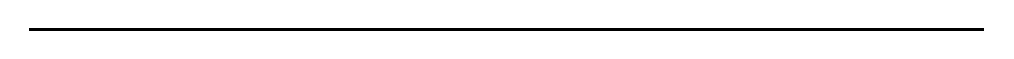
\begin{tikzpicture}
    \draw[very thick](0,0)--(\textwidth,0);
\end{tikzpicture}

% 标题部分
\vspace{-1.0em} % 适当紧凑
{\let\newpage\relax \maketitle}
\thispagestyle{empty} % 确保 \maketitle 后首页依然无页码

% 摘要与关键词
\vspace{-6em} % 紧凑处理
\begin{abstract}
    \songti\zihao{-4} % 设置摘要正文为宋体小四
    这里是摘要的正文内容。cumcmthesis 是为全国大学生数学建模竞赛编写的\LaTeX{}模板，旨在让大家专注于论文的内容写作，而不用花费过多精力在格式的定制和调整上。本手册是相应的参考, 其中提供了一些环境和命令可以让模板的使用更为方便.
    
    \vspace{0.8em}
    \noindent {\songti\zihao{-4}\bfseries 关键词：} {\songti\zihao{-4} 随机森林；STFT；自适应音频处理；数学建模}
\end{abstract}

\newpage % 首页结束，跳转到目录

% --- 目录页：不计页码 ---
\pagestyle{empty}
\tableofcontents
\newpage

% --- 正文页：页码从 1 开始 ---
\pagestyle{plain}
\pagenumbering{arabic}
\setcounter{page}{1}

\section{问题背景与问题重述}
\subsection{问题背景}
这里是正文宋体内容示例。
\subsection{问题重述}

\section{问题分析}
\subsection{研究思路}
\subsection{问题一的分析}

\section{模型假设}

\section{符号说明}
\subsection{名词解释}
\subsection{主要符号说明}

\section{模型建立与求解}
\subsection{问题一模型建立与求解}
\subsubsection{多模态耦合建模体系构建}
\subsubsection{博弈均衡驱动下的智能优化求解与实证验证}

\subsection{问题二模型建立与求解}
\subsubsection{多约束协同优化体系构建}
\subsubsection{智能算法驱动下的动态调控与效益验证}

\subsection{问题三模型建立与求解}
\subsubsection{动态拐点识别与协同优化建模}

\subsection{问题四模型建立与求解}
\subsubsection{数智融合驱动的老城更新决策建模}

\section{灵敏度分析与鲁棒性检验}

\section{模型的评价、改进与推广}
\subsection{模型的优点}
\subsection{模型的缺点} 

\newpage
\section*{参考文献}

\newpage
\section*{附录 1：部分老城街区搬迁优化算法实现}

\end{document}
